%TODO rever referencias
\chapter{2. Testes}
\label{cap:testes}

Testar é uma pratica intrínseca ao desenvolvimento e é antiga a necessidade de
cirar programas para testar cenários específicos~\cite{everett2007}. Testes de 
serão abordados neste cápítulo, iniciando com uma visão geral de testes 
automatizados e conhecendo algumas práticas e padrões utilizados para desenvolver
os mesmos.
%
A automação de testes é uma prática ágil, eficaz e de baixo custo para melhorar
a qualidade dos sistemas de software.

No entanto utilizar testes automatizados 
como uma premissa básica do desenvolvimento é um fenômeno relativamente recente, ]
com início em meados  da década de 1990~\cite{cotter1995}.
%
Além do fato de ser uma técnica bastante utilizada pelas metodologias ágeis
de desenvolvimento.

%------------------------------------------------------------------------------%

\section{Testes Automatizados}

Testes automatizados é a prática de tornar os testes de software independentes da
intervenção humana, criando scripts ou programas simples de computador que exercitam 
o sistema em teste, capturam os efeitos colaterais e fazem verificações, tudo 
automaticamente e dinamicamente~\cite{meszaros2007}.

Os testes automatizados afetam diretamente a qualidade dos sistemas de software,
portanto agregam valor  ao produto final, mesmo que os artefatos adicionais
produzidos não sejam visíveis para os usuários finais do sistemas.
%
Estes testes podem ser divididos em diversos tipo, o que facilita a manutenção 
dos mesmos, coleta de métricas.

\begin{enumerate}

\item \textbf{Testes de unidade:} teste de correção responsável por testar os 
menores trechos de código de um sistema que possui um comportamento definido e 
nomeado.
%
Normalmente, ele é associado a funções para linguagens procedimentais e métodos em 
linguagens orientadas a objetos.
\item \textbf{Testes funcionais:}
%ESCREVER
\item \textbf{Testes de integração:}denominação ampla que representa a busca de 
erros de relacionamento entre quaisquer módulo de um software, incluindo desde 
a integração de pequenas unidades até a integração de bibliotecas das quais um 
sistema depende, servidores e gerenciadores de banco de dados.
\item \textbf{Testes de interface de usuário} testes que verificam a correção 
por meio da simulação de eventos de usuário, a partir destes eventos, são feitas 
verificações na interface e em outras camadas.
\item \textbf{Testes de leiaute:} testes que buscam avaliar a beleza da interface 
e verificar a presença de erros após a renderização, dificeis de indentificar 
com testes comuns de interface
\item \textbf{Testes de aceitação:} são testes de correção e validação, idealmente 
especificados por clientes ou usuários finais do sistema para verificar se um 
modulo funciona como foi especificado~\cite{martin2005}.
%
Testes de aceitação devem utilizar linguagem proxima da natural para evitar 
problemas de interpretação e de ambiguidades~\cite{cunningham2005}.
\item \textbf{Testes de desempenho:} testes que executam trechos do sistema e 
armazenam os tempos de duração obtidos, que ajudam a identificar gargalos que 
precisam de otimização para diminuir o tempo de resposta  para o usuario~\cite{liu2009}.
\item \textbf{Testes de carga:}  teste que exercita o sistema sobre condições de uso 
intenso para avaliar se a infraestrutura é adequada para a expectativa de uso do 
sistema~\cite{avritze1994}.
\item \textbf{Testes de estresse:} teste que visa descobrir os limites do uso da 
infraestrutura, isto é , qual a quantidade máxima de usuários e requisições que o 
sistema consegue antender corretamente e em um tempo aceitável.
\item \textbf{Testes de longevidade:} teste que tem por objetivo encontrar erros 
somente visiveis com um
\item longo tempo de execuçao do sistema, erros que podem ser de cache, replicação, 
execução de serviços agendados, vazamento de memória.
\item \textbf{Testes de segurança:} os testes de segurança servem para verificar se 
os dados ou funcionalidades confidenciais de um sistema  estão protegidos de fraude 
ou de usuários não autorizados. A segurança de um sofware pode envolver aspectos de 
confidenciabilidade, integridade, autenticação, autorização, privacidade~\cite{whittaker2006}.

\end{enumerate}

%------------------------------------------------------------------------------%
\section{Técnicas de Desenvolvimento de testes automatizados}

Automação de testes é uma técnica voltada principalmente para a melhoria de 
qualidade dos sistemas de software. 
%
No processo de desenvolvimento de software é fundamental controlar o custo do 
processo de testes, para isso baterias de testes automatizados devem ser bem 
definidas e implementadas. Assim é importante conhecer boas práticas e técnicas 
de de desenvolvimento de testes automatizados.    
%
Existem várias técnicas de desenvolvimento de software com testes que influenciam 
diretamente na qualidade do sistema. Estas técnicas geralmente possuem um processo 
de atividades pequeno e simples, como TDD e BDD.

\subsection{TDD - Test Driven Development}

Desenvolvimento dirigido por testes, também conhecido como TDD \textit{(Test-Driven Develepment)} 
é uma técnica de desenvolvimento de software que se dá pela repetição dosciplinada 
de um ciclo curto de passos de implementação de testes e do sistema~\cite{koskela2007}.
%
O ciclo de TDD é definido pelos seguintes passos:
%
\begin{enumerate}
\item Implementar um caso de teste;
\item Implementar um trecho do código suficiente para o novo caso de teste ter sucesso 
de tal modo que não quebre os testes previamente escritos;
\item Se necessário, refatorar o código produzido para que ele fique mais organizado;
\end{enumerate}
%
A técnica de desenvolvimento dirigido por testes foi definida por Kent Beck em seu 
livro \textit{Test-Driven Development: By Example}~\cite{beck2002}. Os passos estão 
representados na figura abaixo:
%
\begin{figure}[h]
    \centering
    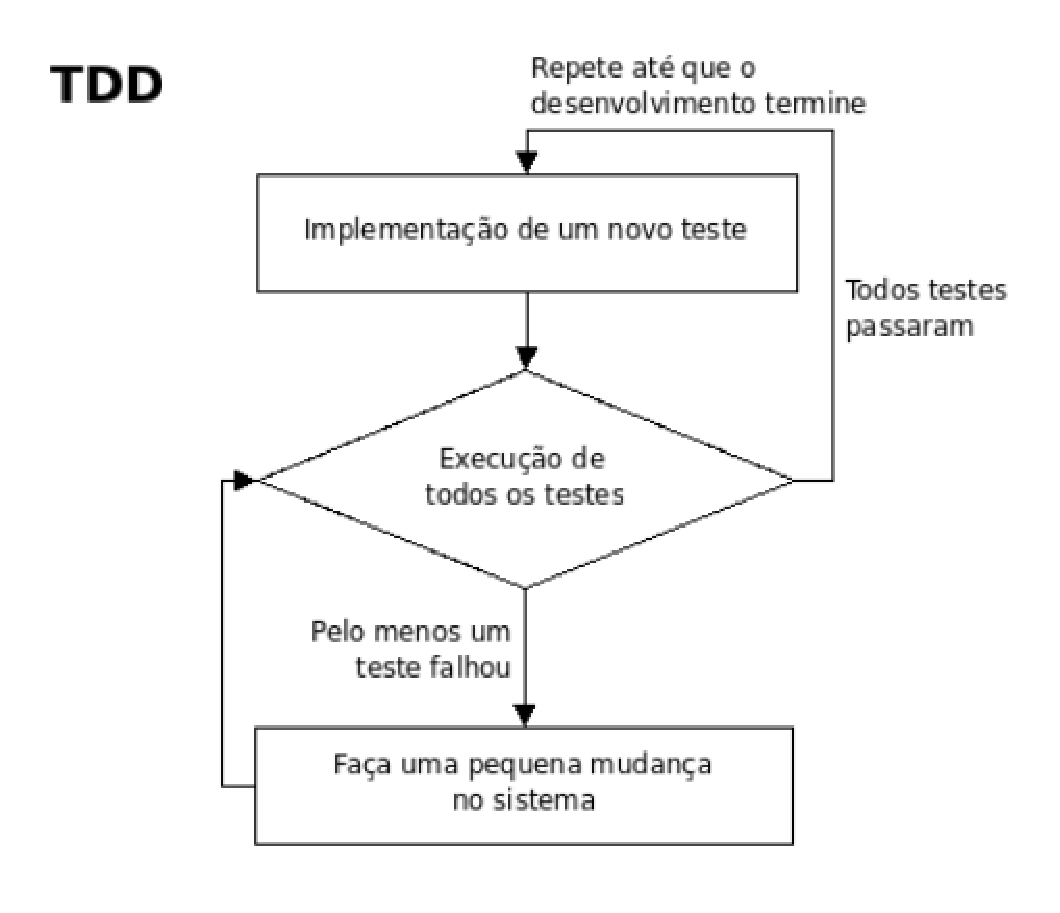
\includegraphics[keepaspectratio=true,scale=0.60]
      {figuras/tdd_ciclo.eps}
    \caption{Ciclo de atividades TDD~\cite{beck2002}}
    \label{tdd_ciclo}
\end{figure}
%

%------------------------------------------------------------------------------%
\subsubsection {Benefícios do TDD}

Uma boa prática do TDD é a bateria de testes, que ajuda o desenvolvedor a evitar 
erros de regreção, quando o desenvolvimento de uma nova funcionalidade quebra uma 
já existente. TDD também tende a contribuir com uma alta cobertura de código, uma 
fez que o desenvolvedor precisa escrever o testes antes da funcionalidade, 
possibilitando a criação de um código mais preciso, coeso e menos acoplado. 
%
Para Massol em \textit{JUnit in Action}, “o objetivo de TDD é ‘código claro que 
funciona’~\cite{massol2003}.
%
TDD propõe o desenvolvimento sempre em pequenos passo, deve-se escrever testes sempre 
para uma menor funcionalidade possível, escrever o código mais simples que faça o 
teste passar e fazer sempre apenas uma refatoração por vez~\cite{beck2002}. Assim o 
desenvolvedor se detém a criar soluções simples, sempre acompanhado de um constante 
feedback dos testes.
%
O ciclo curto de passos definidos por TDD cria uma dependência forte entre codificação 
e testes, o que favorece e facilita a criação de sistemas com alta testabilidade~\cite{bernardo2011}. 
Índices altos de cobertura de código e testabilidade não garantem necessariamente 
qualidade do sistema, mas são métricas bem vistas para sistemas bem desenvolvidos
%
Além de uma técnica de testes automatizados, TDD também é uma prática de desenvolvimento 
de software, pois muda a natureza do processo de codificação, auxiliando na produção 
de um código funcional e limpo.
%
%------------------------------------------------------------------------------%

\subsection{BDD - Behavior Driven Development}
Desenvolvimento dirido por comportamento \textit{(BDD - Behavior Driven Development)} 
é uma prática que recomenda o mesmo ciclo de desenvolvimento de TDD, contudo, induzindo 
a utilização de uma linguagem ubíqua entre cliente e equipe de desenvolvimento~\cite{bernardo2011}, subistituindo termos como assert, \textit{assert, test case, test suite} por termos 
mais comuns ao cliente, como \textit{should, context, specification}
%
O BDD é um processo de desenvolvimento de software baseado no TDD. Embora seja 
principalmente principalmente uma ideia de como um processo de desenvolvimento de 
software deve ser gerenciado. a prática do BDD assume a utilização de ferramentas 
como suporte para o desenvolvimento de software~\cite{haring2011}. O BDD utiliza 
essas ferramentas para que os testes tenham como ponto de partida o compartemento 
dos objetos.
%
O BDD coloca em foco o comportamento em vez da estrutura e faz isso em todos os 
níveis de desenvolvimento. Uma vez que nós reconhecemos isso, ele muda a forma 
como pensamos sobre desenvolvimento para fora do código e começamos a pensar mais 
sobre as intereações sobre pessoas e sistemas, ou entre os objetos, do que sobre a 
estrutura do objeto~\cite{chelimsky2010}.
%
Para que o comportamento seja analisado, é necessário entender o ponto de vista do 
cliente, entendendo o comportamento que o sistema deve ter a partir da visão do cliente. 
%
\subsubsection{Príncipios do BDD}
De acordo com Chelimky, estes são os três príncipios do BDD:
\begin{enumerate}
\item \textbf{O suficiente é suficiente:} parte da ideia de gerenciar o esfoço no 
planejamento inicial do sistema, para não fazer menos nem mais do que o necessário 
para começar, o que se aplica também ao processo de automação.
\item \textbf{Agregar valor as partes interessadas:} Se você está fazendo algo que 
não agrega valor ou que não aumenta a capacidade de agregar valor, pare e faça outra 
coisa em seu lugar.
\item \textbf{Tudo é comportamento:} Do código à aplicação, pode-se usar o mesmo 
pensamento e as mesmas construções linguísticas para descrever o comportamento, em 
qualquer nível de granularidade. 
\end{enumerate}
%
O comportamento do sistema é descrito em historias de usuário, histórias que são 
escritas com a participação tanto de clientes como desemvolvedores do sistema. Assim 
cada hisória de usuário deve seguir, de certa forma, a seguinte estrutura:
%
\textbf{Título:} do que se trata a história.
%
\textbf{Narrativa:} deve identificar as partes interessadas para essa história, as 
funcionalidades requeridas, e o benefício deste comportamento. A narrativa de uma 
história pode ter vários formatos.
%
\textbf{Critério de aceitação:} descrição de cada caso específico da narrativa, 
iniciado pela especificação da condição inicial do cenário, seguidos pelos estados 
que ativam este cenário, finalizado pelos estados esperados ao final do cenário.
%

\subsection{Considerações Finais}
Testes automatizados devem ser desenvolvidos com prioridade, buscando um rápido 
\textit{feedback}, contribuindo assim com a melhoria do sistema. Para isso é 
necessário que os cenários de testes estejam bem definidos junto à equipe.
%
